\documentclass[12pt]{article}
\usepackage{url}
\usepackage[spanish, english]{babel}
\selectlanguage{spanish}
\usepackage[fixlanguage]{babelbib}
\selectbiblanguage{spanish}
\usepackage{url}
\usepackage[utf8]{inputenc}
\usepackage{float}
\usepackage{fullpage}
\usepackage{amsmath}
\usepackage{amssymb}
\usepackage{graphicx}
\usepackage{verbatim} 
\usepackage{caption, subcaption}
\usepackage{tikz}%Generar plots
\usepackage{pgfplots}%Generar plots
\pgfplotsset{compat=1.5}
\usepackage{pgfplotstable,filecontents}
\pgfplotsset{compat=1.9}% supress warning
\usepackage{booktabs}

\pgfkeys{/pgf/number format/.cd,fixed,precision=5}

\usepackage[titletoc, title]{appendix}
\addto{\captionsspanish}{\renewcommand*{\appendixname}{Anexo}}

\bibliographystyle{bababbrv}

\title{Segmentación de Piel}
\author{Jorge Bahamonde, Sebastián González\\
\small{\url{jbahamon@ug.uchile.cl}, \url{segonzal@dcc.uchile.cl}}}
\date{}

\begin{document}
\maketitle

\begin{abstract}
    El reconocimiento y clasificación de caracteres impresos es un método
    conocido para la digitalización de texto, de modo de poder realizar el
    almacenamiento, búsqueda y otros análisis de mejor forma.  El estudio y
    icomparación de diferentes descriptores es necesario en un área en que
    diversas variantes son propuestas en base a intuiciones. En particular, una
    clase importante de descriptores está compuesta por aquellos basados en
    nociones de concavidad. En este trabajo se estudiaron tres descriptores
    basados en concavidad para el caso de la clasificación de dígitos impresos.
    Se exploró (de forma limitada) el espacio de parámetros del clasificador
    utilizado (KNN). Posteriormente, se analizó la extensión de los resultados
    obtenidos en el caso de agregar mecanismos de división espacial en la
    obtención de los descriptores, buscando comparar el comportamiento de éstos.
\end{abstract}

\section{Introducción}

%> grandes data sets (WWW) hacen posible soportar simples, eficientes algoritmos de aprendizaje.
%> dado una gran cantidad de datos, incluso simples reglas de aprendizaje arrojan buenos resultados
%> importante en el aprendizaje visual es la construccion de modelos de apariencia de la imagen desde datos de pixeles
% en paper "Statistical color models with application to skin detection" entrenaron un modelo de mix_of_gaussians con MUUUUUUCHOS dataz para clasificacion de piel
% analizamos la performance de MoG en el reconocimiento de piel en un set de 30 imagenes sacadas de la web

La masificación en el uso de la World Wide Web ha contribuido en la aparición de
grandes conjuntos de datos. La masividad de datos disponible soprta la aparición de
algoritmos simples y computacionalmente eficientes.Las grandes colecciones de imágenes on-line permiten
la construcción de modelos estadísticos, caracterizando la apariencia de una imagen utilizando
la información de sus pixeles.

La segmentación de piel es una aplicación útil del reconocimiento de patrones. Es utilizada en el campo de la detección de personas y rostros, generalmente
para discriminar ambigüedades en la detección y reducir malas clasificaciones. En el ámbito de la seguirdad, ha sido usada en programas de control parental, como herramienta de detección de contenido adulto en la web.

Estudiamos el segmentador de piel probabilístico propuesto por \emph{Jones y Rehg} en \emph{Statistical color models with application to skin detection}. En particular analizamos el desempeño del método \emph{Mixture of Gaussians}, al variar la razón de costo asociado a los falsos positivos y falsos negativos.

Utilizamos un set de datos de treinta imágenes, de las cuales la mitad fueron encontradas en internet seleccionadas, considerando la tez de los sujetos. La segunda mitad consiste en imágenes extraidas del dataset Pratheepan.



\section{Descripción del Trabajo}

En este trabajo se realizó la evaluación de un algoritmo para el reconocimiento
de piel basado en modelos estadísticos de color. 

\subsection{Modelos de color}

Una forma de modelar una característica a detectar es mediante un modelo
estadístico sobre los colores de la imagen. Un pixel con cierto valor $rgb$ es
clasificado por uno de estos modelos como ser efectivamente piel si:

\begin{equation}
    \frac{ \mathbb{P} [ rgb|skin ] }{ \mathbb{P} [ rgb | \neg skin ] } \geq
    \Theta
\end{equation}

con $\Theta$ un umbral que puede ser descrito como función del costo de tener
falsos positivos y falsos negativos:

\begin{equation}
    \Theta = \frac{c_p \mathbb{P} [\neg skin]}{c_n \mathbb{P}[skin]}
\end{equation}

Ahora bien, las distribuciones $\mathbb{P} [ rgb|skin ]$ y $\mathbb{P} [ rgb | \neg
skin ]$ pueden ser determinadas de distintas formas. En el caso de este trabajo, se
utilizó un modelo que describe estas distribuciones como una combinación de
funciones gaussianas.

\subsection{Modelo basado en Mezcla de Gaussianas}

Una forma de modelar las distribuciones de probabilidad  $\mathbb{P} [ rgb|skin
]$ y $\mathbb{P} [ rgb | \neg skin ]$ es mediante una suma de funciones
gaussianas:

\begin{equation}
    \mathbb{P}[\mathbf{x}] = \sum\limits_{i=1}^N w_i
    \frac{1}{(2\pi)^{\frac{3}{2}} | \Sigma_i |^\frac{1}{2}} e^{-\frac{1}{2}
    (\mathbf{x} - \mathbf{\mu}_i)^{\text{T}} \Sigma_i ^{-1} (\mathbf{x} -
    \mathbf{\mu}_i)},
\end{equation} 

donde los valores $\mu_i$ y $\Sigma_i$ son las medias de cada gaussiana y las
correspondientes matrices (diagonales) de covarianza. Los valores $w_i$
determinan el peso que cada gaussiana ejerce en la mezcla. $N$ define la
complejidad del modelo, (ya que un mayor valor de $N$ resulta en más gaussianas
y por tanto un mayor número de grados de libertad) siendo un parámetro a
elección. 

Los autores de \cite{skin} entrenaron modelos para estimar ambas
distribuciones de probabilidad descritas, con lo que estos parámetros tienen
valores dados. Así, el trabajo se enfocó en variar el umbral de detección,
$\Theta$.

\subsection{Dataset utilizado}

Se construyó un pequeño \emph{dataset} compuesto por imágenes de dos tipos. Por
un lado, se recopilaron 15*** imágenes intentando incorporar variaciones en
iluminación, tonos de piel y el nivel de detalle del fondo. Otras 15 imágenes
fueron tomadas de un dataset***. Para cada imagen del dataset generado, se
obtuvo una imagen que identifica las zonas que son piel, generándose así la
\emph{ground truth} contra la que se comparó el rendimiento del modelo
estadístico.

\begin{figure}[h]
    \centering
    \hfill\subcaptionbox{Imagen del \emph{dataset}
    utilizado.}{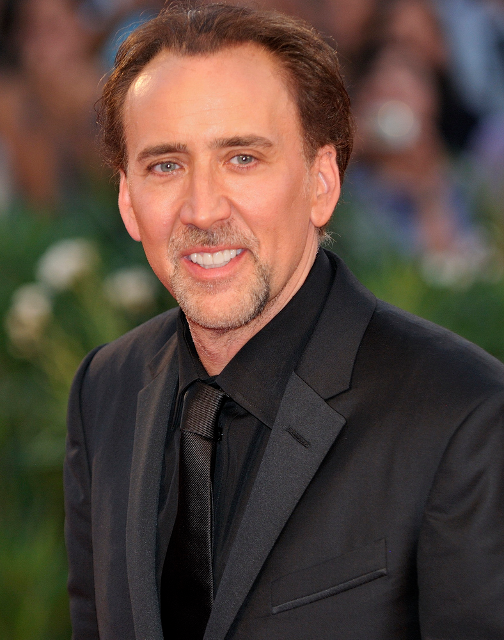
\includegraphics[scale=0.9]{../images/nonbin/12.png}}
    \hfill\subcaptionbox{Perfil de piel utilizado como \emph{ground
    truth}}{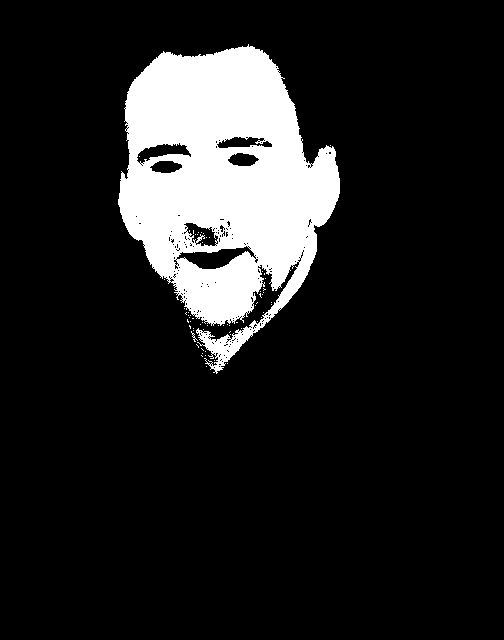
\includegraphics[scale=0.9]{../images/bin/12.png}}
    \caption{Ejemplo del \emph{dataset} usado.}
\end{figure}

\section{Resultados obtenidos}

Para evaluar el desempeño del modelo estudiado, se le utilizó para detectar piel
en las imágenes del dataset, contrastándolos con los perfiles de piel
etiquetados correctamente. 

Se definen, en este contexto: 

\begin{itemize}
    \item el \textbf{número de positivos ($P$)} como el número de pixeles en el dataset
        que corresponden a piel (según la \emph{ground truth});
    \item el \textbf{número de negativos($N$)} como el número de pixeles en el dataset
        que no corresponden a piel;
    \item el \textbf{número de falsos positivos ($FP$)} como el número de
        pixeles en el dataset que el modelo identifica como piel, pero que no
        están etiquetados como tal en la \emph{ground truth};
    \item el \textbf{número de verdaderos positivos ($TP$)} como el número de
        pixeles en el dataset que el algoritmo identifica correctamente como
        piel;
    \item la \textbf{tasa de verdaderos positivos ($TPR$)} (también llamada
        probabilidad de detección correcta) como $\frac{TP}{P}$;
    \item la \textbf{tasa de falsos positivos ($FPR$)} (o probabilidad de
        detección incorrecta) como $FP/N$.
\end{itemize}

Así, el comportamiento de un modelo de detección como el estudiado puede ser
apreciado al comparar el comportamiento de la $FPR$ versus la $TPR$. La curva
definida por estas dos variables al variar un tercer parámetro se denomina curva
ROC (del inglés \emph{receiver operating characteristic}). Esta curva muestra
cuán apropiado puede ser un modelo o algoritmo para ciertas aplicaciones, ya que
el costo de un falso positivo versus un verdadero positivo varía dependiendo del
contexto.

Se construyó una curva ROC a partir de los resultados obtenidos al utilizar el modelo de mezcla
de gaussianas en el dataset generado y la posterior comparación con la
\emph{ground truth}:


\begin{figure}[h]
    \centering
   % \includegraphics{digit}

\begin{tikzpicture}
\begin{axis}[
	title=ROC,
	xlabel={False Positive Rate},
	ylabel={True Positive Rate},
	grid=major,
%	legend entries={$0.01$ , $0.1$,$0.5$},
%	legend style={at={(0,1)},anchor=north west},
]
\addplot table [only marks,scatter,x={FP}, y={TP}]{results.csv};
%\addplot table [only marks,scatter,x={FP}, y={TP}]{results(0.1,1,0.1).csv};
%\addplot table [only marks,scatter,x={FP}, y={TP}]{results(0.1,1,0.5).csv};
\end{axis}
\end{tikzpicture}
    \caption{Curva ROC obtenida al variar el parámetro umbral $\Theta \in \{ 0.1,0.5,...,0.9,0.91,...0,99\}$.}
\end{figure}

Para ejemplificar de mejor forma el comportamiento del algoritmo, se presentan a
continuación algunos ejemplos en los que el modelo muestra diferentes grados de
efectividad.

\begin{figure}[h]
    \centering
   \hfill\subcaptionbox{Imagen original}{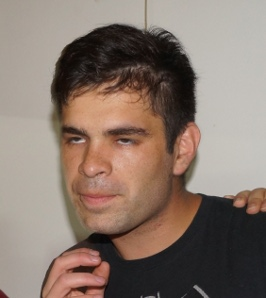
\includegraphics[scale=0.4]{../images/nonbin/05.png}}
   \hfill\subcaptionbox{\emph{GroundTruth}.}{
\includegraphics[scale=0.4]{../images/bin/05.png}}
   \hfill\subcaptionbox{Output de \emph{Mixture of Gaussians} con $\Theta = 0.5$.}{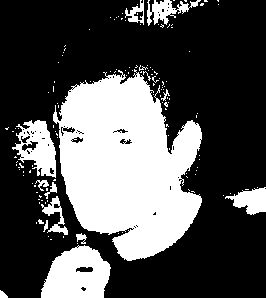
\includegraphics[scale=0.4]{../done0.5/05.png}}
   \hfill\subcaptionbox{Output de \emph{MoG} con $\Theta = 0.9$.}{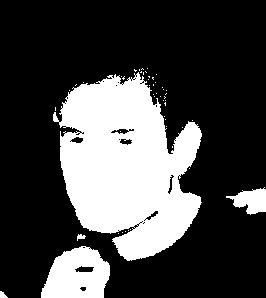
\includegraphics[scale=0.4]{../done0.9/05.png}}
    \caption{A la izquierda, imágenes del dataset. En el centro, la \emph{ground
    truth} correspondiente. A la derecha, el resultado obtenido por el modelo de
    mezcla de gaussianas.}
\end{figure}

\subsection{Discusión}

Se observa que, en general, el modelo alcanza **. En particular, el modelo
parece presentar un menor rendimiento cuando ***, logrando, por el contrario, un
mejor comportamiento en el caso de ***. 

Por otro lado, se aprecia que existen diferentes tipos de error. En ciertos
casos, existen muchos pixeles dispersos detectados como piel esparcidos por la
imagen. En este caso, aplicar algún mecanismo de detección de \emph{blobs}
podría ayudar a descartar este tipo de errores. Otros casos corresponden a la
identificación de ciertas telas y texturas como piel, en los que complementar
con técnicas como \emph{local binary patterns} podrían ayudar a un mejor
desempeño. De todos modos, la conveniencia de complementar el modelo con estas
herramientas depende del contexto de uso.

\section{Conclusiones}



\selectlanguage{spanish}
\selectbiblanguage{spanish}

\bibliography{./informe}

%\begin{appendices}

\section{Matrices de confusión para descriptores sin división espacial}

Se incluyen aquí las matrices de confusión para los descriptores que no
consideran división espacial. Cada columna de la matriz representa el porcentaje
de instancias en una clase predicha; cada fila representa el porcentaje de
instancias en una clase real. Las columnas y filas de cada matriz están
ordenadas de izquierda a derecha y de arriba a abajo: así, la primera fila
corresponde al 0, y la última al 9, por ejemplo.

El valor de p mencionado es el orden de la distancia de Minkowski utilizada.
Así, un valor de 1 resulta en la distancia de Manhattan, mientras que un valor
de 2 resulta en la distancia Euclidiana. El valor de K corresponde al número de
vecinos considerados para el algoritmo de \emph{K-nearest neighbors}.

\subsection{Descriptor 4CC}

\subsubsection*{p = 1, K = 1}

$$\begin{pmatrix}
96.72&0.0&0.0&0.0&0.0&0.0&0.66&0.0&2.3&0.33\\
0.0&95.74&0.66&0.0&0.0&1.31&0.0&2.3&0.0&0.0\\
0.0&1.64&90.16&3.28&0.33&3.61&0.0&0.0&0.33&0.66\\
0.0&0.0&2.62&92.13&0.0&1.64&0.0&0.0&1.31&2.3\\
0.0&0.33&0.33&0.0&97.7&0.33&0.98&0.33&0.0&0.0\\
0.0&0.0&3.93&2.3&0.33&91.48&0.98&0.98&0.0&0.0\\
4.26&0.0&0.0&0.0&0.98&0.33&91.48&0.0&1.31&1.64\\
0.0&0.33&0.0&0.33&0.0&0.66&0.0&98.36&0.0&0.33\\
8.2&0.0&0.0&0.0&0.0&0.98&1.64&0.0&88.2&0.98\\
1.97&0.0&0.0&1.97&0.0&0.0&0.66&0.0&2.62&92.79
\end{pmatrix}$$

\subsubsection*{p = 1, K = 5}

$$\begin{pmatrix}
96.39&0.0&0.0&0.0&0.0&0.0&0.98&0.0&2.3&0.33\\
0.0&93.77&2.62&0.0&0.0&2.3&0.0&0.98&0.0&0.33\\
0.33&2.3&85.9&2.95&1.31&5.57&0.0&0.0&0.98&0.66\\
0.33&0.98&5.9&85.57&0.66&2.3&0.0&0.33&1.64&2.3\\
0.66&2.62&1.31&0.0&94.43&0.33&0.33&0.33&0.0&0.0\\
0.0&1.31&5.9&2.3&0.0&88.85&0.98&0.33&0.33&0.0\\
4.92&0.33&0.0&0.0&0.66&1.31&89.18&0.0&3.28&0.33\\
0.33&0.66&0.0&0.66&0.0&0.66&0.0&97.38&0.0&0.33\\
10.49&0.0&0.0&0.0&0.33&0.98&3.28&0.0&83.93&0.98\\
3.61&0.33&0.66&1.97&0.33&0.33&0.33&0.33&2.3&89.84
\end{pmatrix}$$

\subsubsection*{p = 1, K = 10}
$$\begin{pmatrix}
96.72&0.0&0.0&0.0&0.0&0.0&0.98&0.0&2.3&0.0\\
0.0&92.46&2.62&0.0&0.0&2.3&0.0&2.62&0.0&0.0\\
0.66&1.97&85.25&1.97&0.98&6.23&0.98&0.0&0.98&0.98\\
0.66&0.66&7.54&83.61&0.33&3.28&0.0&0.33&1.31&2.3\\
0.98&1.64&0.98&0.0&94.43&0.33&0.33&0.66&0.0&0.66\\
0.0&0.66&4.26&0.98&0.33&91.15&0.66&1.64&0.33&0.0\\
4.59&0.33&0.0&0.0&1.64&0.98&89.51&0.0&2.95&0.0\\
0.33&1.31&0.0&0.33&0.0&1.31&0.0&96.72&0.0&0.0\\
10.82&0.0&0.0&0.33&0.0&0.33&3.28&0.0&83.61&1.64\\
2.95&0.33&0.0&0.98&0.66&0.33&0.33&0.66&4.26&89.51
\end{pmatrix}$$

\subsubsection*{p = 1, K = 20}
$$\begin{pmatrix}
95.41&0.0&0.0&0.0&0.0&0.0&0.0&0.0&4.59&0.0\\
0.0&90.16&3.28&0.33&0.0&2.95&0.0&3.28&0.0&0.0\\
0.33&0.98&83.28&3.93&0.98&7.21&0.66&0.0&0.66&1.97\\
1.64&0.98&5.57&82.62&0.0&3.93&0.0&0.33&0.98&3.93\\
1.31&1.97&1.64&0.0&92.46&0.98&0.33&0.33&0.33&0.66\\
0.33&1.31&5.57&0.66&0.33&88.85&0.98&1.64&0.33&0.0\\
5.9&0.33&0.0&0.0&1.64&0.66&88.52&0.0&2.95&0.0\\
0.33&1.31&0.0&0.0&0.0&1.97&0.0&96.39&0.0&0.0\\
10.49&0.33&0.0&0.0&0.33&0.33&1.64&0.33&85.25&1.31\\
5.25&0.0&0.33&0.33&0.0&0.0&0.98&0.66&4.26&88.2
\end{pmatrix}$$

\subsubsection*{p = 2, K = 1}
$$\begin{pmatrix}
94.75&0.0&0.0&0.0&0.0&0.0&0.66&0.0&4.59&0.0\\
0.0&95.41&0.66&0.98&0.0&0.98&0.0&1.64&0.0&0.33\\
0.0&0.66&87.87&4.59&0.33&4.92&0.0&0.0&0.98&0.66\\
0.0&0.0&3.61&90.82&0.0&1.97&0.0&0.0&0.33&3.28\\
0.0&0.66&0.0&0.0&96.39&0.98&1.31&0.0&0.33&0.33\\
0.0&0.0&4.59&1.64&0.33&91.48&0.98&0.98&0.0&0.0\\
2.62&0.0&0.0&0.0&1.31&0.33&91.8&0.0&3.93&0.0\\
0.0&0.0&0.0&0.66&0.0&0.33&0.0&98.69&0.0&0.33\\
6.89&0.0&0.0&0.33&0.0&0.98&2.95&0.0&87.54&1.31\\
1.64&0.0&0.0&2.62&0.0&0.33&0.33&0.33&2.3&92.46
\end{pmatrix}$$

\subsubsection*{p = 2, K = 5}
$$\begin{pmatrix}
94.1&0.0&0.0&0.0&0.0&0.0&0.98&0.0&4.59&0.33\\
0.0&94.43&1.31&0.0&0.0&2.62&0.0&1.31&0.0&0.33\\
0.0&1.64&83.28&4.92&1.31&6.56&0.33&0.0&1.31&0.66\\
0.33&1.31&7.54&83.93&0.0&1.64&0.0&0.33&0.98&3.93\\
0.98&1.97&0.98&0.33&94.1&0.66&0.0&0.0&0.33&0.66\\
0.0&1.31&7.54&0.33&0.66&87.87&1.31&0.66&0.33&0.0\\
3.93&0.0&0.66&0.0&0.98&1.64&87.54&0.0&4.92&0.33\\
0.0&0.66&0.33&0.66&0.0&0.66&0.0&97.38&0.0&0.33\\
10.49&0.0&0.0&0.0&0.98&0.98&4.26&0.0&81.97&1.31\\
1.64&0.33&0.0&1.64&0.33&0.98&0.98&0.66&3.61&89.84
\end{pmatrix}$$

\subsubsection*{p = 2, K = 10}
$$\begin{pmatrix}
93.77&0.0&0.0&0.0&0.0&0.0&0.66&0.0&5.57&0.0\\
0.0&92.46&1.97&0.33&0.0&2.95&0.0&2.3&0.0&0.0\\
0.33&1.31&83.61&2.95&1.31&7.21&0.98&0.0&0.98&1.31\\
0.33&0.66&8.52&82.62&0.33&2.62&0.0&0.33&0.66&3.93\\
0.98&1.97&1.64&0.0&93.44&0.66&0.33&0.0&0.33&0.66\\
0.0&0.33&5.9&1.31&0.33&88.52&1.31&1.64&0.66&0.0\\
4.92&0.33&0.66&0.0&0.98&0.66&87.21&0.0&5.25&0.0\\
0.0&1.31&0.0&0.0&0.0&0.98&0.33&97.05&0.0&0.33\\
15.08&0.0&0.0&0.0&0.66&0.33&1.97&0.33&78.69&2.95\\
2.95&0.66&0.33&0.98&0.0&0.33&1.31&0.33&3.28&89.84
\end{pmatrix}$$

\subsubsection*{p = 2, K = 20}
$$\begin{pmatrix}
92.46&0.0&0.0&0.0&0.0&0.0&0.0&0.0&7.21&0.33\\
0.0&91.8&2.3&0.33&0.0&3.61&0.0&1.97&0.0&0.0\\
0.33&1.97&80.33&3.93&1.31&7.87&0.66&0.0&1.31&2.3\\
1.31&0.66&6.56&82.3&0.33&3.28&0.0&0.33&0.66&4.59\\
1.31&1.64&1.31&0.0&92.79&0.98&0.66&0.33&0.33&0.66\\
0.33&0.98&7.21&1.31&0.33&86.56&1.64&0.98&0.33&0.33\\
6.56&0.33&0.33&0.0&1.31&1.97&85.57&0.0&3.93&0.0\\
0.98&1.64&0.0&0.0&0.0&1.97&0.0&95.41&0.0&0.0\\
14.75&0.0&0.33&0.33&0.33&0.66&2.95&0.33&77.38&2.95\\
4.26&0.33&0.33&0.98&1.31&0.33&1.31&0.33&2.95&87.87
\end{pmatrix}$$

\subsection{Descriptor 8CC}
\subsubsection*{p = 1, K = 1}
$$\begin{pmatrix}
91.8&0.0&0.0&0.0&0.0&0.33&5.57&0.0&1.31&0.98\\
0.0&97.38&0.66&0.33&0.0&0.0&0.0&0.98&0.0&0.66\\
0.0&0.66&98.03&0.66&0.0&0.0&0.0&0.0&0.33&0.33\\
0.0&0.0&0.0&96.07&0.0&2.95&0.0&0.33&0.0&0.66\\
0.0&0.0&0.0&0.0&98.69&0.33&0.0&0.0&0.0&0.98\\
0.66&0.0&0.0&1.64&0.0&91.48&0.0&0.66&2.3&3.28\\
12.79&0.66&0.0&0.0&0.0&0.0&84.26&0.0&0.98&1.31\\
0.0&0.33&0.0&0.66&0.0&0.0&0.0&99.02&0.0&0.0\\
4.92&0.0&0.0&0.33&0.0&0.33&1.97&0.0&91.15&1.31\\
0.98&0.0&0.0&0.0&0.0&0.98&0.33&0.0&3.93&93.77
\end{pmatrix}$$

\subsubsection*{p = 1, K = 5}
$$\begin{pmatrix}
91.8&0.0&0.0&0.33&0.0&0.33&5.57&0.0&1.31&0.66\\
0.0&95.41&2.62&0.0&0.33&0.33&0.0&0.66&0.0&0.66\\
0.0&1.31&97.7&0.33&0.0&0.0&0.0&0.0&0.66&0.0\\
0.33&0.33&0.66&94.43&0.0&2.3&0.0&0.66&0.66&0.66\\
0.0&0.0&0.0&0.0&97.38&0.98&0.66&0.0&0.0&0.98\\
1.31&0.33&0.0&2.95&0.0&88.2&0.33&0.98&2.62&3.28\\
12.79&0.66&0.0&0.0&0.33&0.33&83.93&0.0&1.64&0.33\\
0.0&0.66&0.98&0.66&0.0&0.0&0.0&97.7&0.0&0.0\\
5.25&0.0&0.0&0.33&0.0&0.66&3.28&0.0&87.54&2.95\\
0.66&0.0&0.33&0.0&1.64&0.98&0.66&0.33&3.93&91.48
\end{pmatrix}$$

\subsubsection*{p = 1, K = 10}
$$\begin{pmatrix}
92.13&0.0&0.0&0.0&0.0&0.66&4.92&0.0&1.31&0.98\\
0.0&95.74&2.62&0.33&0.0&0.66&0.0&0.66&0.0&0.0\\
0.0&2.62&95.74&0.33&0.0&0.33&0.0&0.0&0.66&0.33\\
0.66&0.66&1.31&93.11&0.0&1.64&0.0&0.98&0.66&0.98\\
0.66&0.66&0.0&0.0&95.08&0.98&1.64&0.0&0.0&0.98\\
1.31&0.98&0.0&1.64&0.0&86.23&0.33&0.66&3.28&5.57\\
14.75&0.66&0.0&0.0&0.33&0.33&80.0&0.0&3.28&0.66\\
0.0&0.66&0.66&0.66&0.0&0.0&0.0&98.03&0.0&0.0\\
4.92&0.0&0.0&0.33&0.0&0.66&3.28&0.0&89.18&1.64\\
1.31&0.0&0.33&0.0&1.64&0.33&0.66&0.66&5.57&89.51
\end{pmatrix}$$

\subsubsection*{p = 1, K = 20}
$$\begin{pmatrix}
89.51&0.0&0.0&0.0&0.0&0.66&6.56&0.0&1.97&1.31\\
0.0&92.13&4.92&0.0&0.0&0.66&0.0&1.31&0.0&0.98\\
0.0&3.93&94.43&0.0&0.0&0.0&0.33&0.0&0.98&0.33\\
0.66&0.66&1.97&91.48&0.0&1.97&0.0&0.98&0.98&1.31\\
1.64&2.3&0.0&0.0&92.79&0.98&1.31&0.0&0.33&0.66\\
1.64&1.64&0.0&1.31&0.0&83.61&0.0&0.33&5.25&6.23\\
17.05&0.66&0.0&0.0&0.33&0.33&77.38&0.0&3.61&0.66\\
0.0&0.98&0.98&0.33&0.0&0.0&0.0&97.38&0.0&0.33\\
4.26&0.0&0.0&0.33&0.0&0.98&2.62&0.0&87.87&3.93\\
1.64&0.0&0.33&0.0&1.64&0.66&0.0&0.33&5.57&89.84
\end{pmatrix}$$

\subsubsection*{p = 2, K = 1}
$$\begin{pmatrix}
89.84&0.0&0.0&0.0&0.0&0.66&7.87&0.0&0.98&0.66\\
0.0&96.07&1.97&0.33&0.33&0.0&0.0&0.66&0.0&0.66\\
0.0&1.31&97.38&0.98&0.0&0.0&0.0&0.0&0.33&0.0\\
0.0&0.0&0.66&94.75&0.0&3.28&0.0&0.33&0.0&0.98\\
0.33&0.0&0.0&0.0&98.03&0.66&0.33&0.0&0.0&0.66\\
0.33&0.33&0.0&2.95&0.0&91.15&0.0&0.66&1.31&3.28\\
12.46&0.66&0.0&0.0&0.33&0.0&84.26&0.0&0.98&1.31\\
0.0&0.33&0.0&0.66&0.0&0.0&0.0&99.02&0.0&0.0\\
4.26&0.0&0.0&0.33&0.33&0.66&2.3&0.0&90.49&1.64\\
0.98&0.0&0.0&0.0&0.0&0.66&0.0&0.0&4.26&94.1
\end{pmatrix}$$

\subsubsection*{p = 2, K = 5}
$$\begin{pmatrix}
89.18&0.0&0.0&0.33&0.0&0.66&7.87&0.0&1.31&0.66\\
0.0&94.43&2.62&0.0&0.33&0.66&0.0&0.98&0.0&0.98\\
0.0&1.97&96.39&0.98&0.0&0.0&0.0&0.0&0.66&0.0\\
0.66&0.33&1.31&92.46&0.0&2.95&0.0&0.66&0.98&0.66\\
0.0&0.0&0.0&0.0&97.7&0.66&0.66&0.0&0.0&0.98\\
1.64&1.64&0.0&3.61&0.0&86.89&0.0&0.66&1.97&3.61\\
13.11&0.66&0.0&0.0&0.33&0.33&83.28&0.0&1.64&0.66\\
0.0&0.66&0.66&0.66&0.0&0.0&0.0&98.03&0.0&0.0\\
4.92&0.0&0.0&0.33&0.0&1.97&4.26&0.0&86.89&1.64\\
0.98&0.0&0.66&0.0&1.64&1.31&0.0&0.66&4.26&90.49
\end{pmatrix}$$

\subsubsection*{p = 2, K = 10}
$$\begin{pmatrix}
90.16&0.0&0.0&0.0&0.0&0.66&6.23&0.0&1.97&0.98\\
0.0&93.11&3.93&0.0&1.31&0.66&0.0&0.66&0.0&0.33\\
0.0&2.62&95.41&0.66&0.0&0.66&0.0&0.0&0.33&0.33\\
0.66&0.66&0.98&90.82&0.0&3.93&0.0&0.98&0.98&0.98\\
0.33&1.31&0.0&0.0&95.08&0.98&0.98&0.0&0.33&0.98\\
1.31&0.98&0.0&4.26&0.0&83.28&0.33&0.98&3.28&5.57\\
14.75&0.66&0.0&0.0&0.66&0.98&79.67&0.0&2.95&0.33\\
0.0&1.31&0.66&0.66&0.0&0.0&0.0&97.38&0.0&0.0\\
3.93&0.33&0.0&0.33&0.0&1.31&3.61&0.0&87.54&2.95\\
1.64&0.0&0.66&0.0&1.64&0.66&0.0&0.66&4.59&90.16
\end{pmatrix}$$

\subsubsection*{p = 2, K = 20}
$$\begin{pmatrix}
86.56&0.0&0.0&0.0&0.0&0.66&8.85&0.0&2.62&1.31\\
0.0&89.84&6.23&0.0&0.33&0.98&0.0&0.98&0.0&1.64\\
0.0&5.25&92.13&0.66&0.33&0.66&0.0&0.0&0.66&0.33\\
0.66&0.98&1.64&88.85&0.0&4.92&0.0&0.98&0.98&0.98\\
0.98&2.62&0.0&0.0&92.13&0.98&1.97&0.0&0.33&0.98\\
1.31&1.97&0.33&4.26&0.0&81.31&0.0&0.33&4.92&5.57\\
16.72&0.66&0.0&0.0&0.98&0.98&76.72&0.0&3.28&0.66\\
0.0&0.98&0.98&0.98&0.0&0.0&0.0&96.72&0.0&0.33\\
3.28&0.0&0.0&0.33&0.0&1.31&3.61&0.0&86.23&5.25\\
1.97&0.0&0.66&0.0&1.64&1.31&0.0&0.33&5.57&88.52
\end{pmatrix}$$

\subsection{Descriptor 13C}

\subsubsection*{p = 1, K = 1}
$$\begin{pmatrix}
97.38&0.0&0.0&0.0&0.0&0.0&0.0&0.0&2.62&0.0\\
0.0&96.72&0.66&0.0&0.33&0.0&0.0&1.97&0.0&0.33\\
0.0&2.3&95.41&0.0&0.33&0.98&0.33&0.0&0.33&0.33\\
0.0&0.0&0.0&98.36&0.0&0.66&0.0&0.0&0.0&0.98\\
0.33&0.0&0.0&0.0&97.7&0.0&0.0&0.0&1.31&0.66\\
0.0&0.98&0.98&0.33&0.33&96.39&0.0&0.66&0.0&0.33\\
0.33&0.0&0.0&0.0&0.66&0.0&99.02&0.0&0.0&0.0\\
0.0&0.66&0.0&0.0&0.0&0.0&0.0&99.34&0.0&0.0\\
3.93&0.0&0.0&0.0&0.66&0.33&1.64&0.0&93.44&0.0\\
0.33&0.0&0.33&0.33&0.0&0.0&0.33&0.0&0.33&98.36
\end{pmatrix}$$

\subsubsection*{p = 1, K = 5}

$$\begin{pmatrix}
96.72&0.0&0.0&0.0&0.0&0.0&0.0&0.0&3.28&0.0\\
0.0&95.08&0.98&0.0&0.33&1.64&0.0&1.64&0.0&0.33\\
0.0&3.61&93.44&0.0&0.0&0.66&0.33&0.0&0.98&0.98\\
0.0&1.97&0.33&96.07&0.0&0.0&0.0&0.33&0.0&1.31\\
0.66&0.98&0.0&0.0&96.07&0.33&0.0&0.0&0.66&1.31\\
0.0&1.97&1.64&1.31&0.0&93.77&0.0&0.98&0.0&0.33\\
1.31&0.33&0.0&0.0&0.66&0.0&97.38&0.0&0.33&0.0\\
0.0&0.98&0.0&0.0&0.0&0.33&0.0&98.69&0.0&0.0\\
4.92&0.0&0.0&0.0&0.98&0.33&2.3&0.0&91.15&0.33\\
0.66&0.98&0.33&0.98&0.0&0.0&0.0&0.33&0.66&96.07
\end{pmatrix}$$

\subsubsection*{p = 1, K = 10}
$$\begin{pmatrix}
97.7&0.0&0.0&0.0&0.0&0.0&0.0&0.0&2.3&0.0\\
0.0&95.41&0.98&0.0&0.33&1.64&0.0&1.31&0.0&0.33\\
0.0&4.26&91.8&0.0&0.0&0.33&1.31&0.0&1.31&0.98\\
0.0&1.64&0.0&94.75&0.0&1.64&0.0&0.33&0.0&1.64\\
0.66&0.66&0.33&0.0&95.74&0.33&0.0&0.0&0.33&1.97\\
0.0&2.62&1.97&1.31&0.0&93.11&0.0&0.66&0.0&0.33\\
0.33&0.33&0.0&0.0&0.98&0.0&98.03&0.0&0.33&0.0\\
0.0&2.62&0.0&0.0&0.0&0.33&0.0&97.05&0.0&0.0\\
4.92&0.0&0.0&0.0&0.66&0.33&2.3&0.0&91.48&0.33\\
1.31&0.98&0.33&0.98&0.0&0.0&0.0&0.33&0.98&95.08
\end{pmatrix}$$

\subsubsection*{p = 1, K = 20}
$$\begin{pmatrix}
96.39&0.0&0.0&0.0&0.0&0.0&0.0&0.0&3.61&0.0\\
0.0&95.74&0.98&0.0&0.0&1.97&0.0&0.98&0.0&0.33\\
0.0&2.95&91.8&0.33&0.0&0.98&1.31&0.0&1.31&1.31\\
0.0&2.3&0.0&94.1&0.0&1.31&0.0&0.33&0.0&1.97\\
0.66&1.97&0.0&0.0&94.75&0.33&0.0&0.0&0.66&1.64\\
0.0&2.95&1.64&0.98&0.0&93.44&0.0&0.66&0.0&0.33\\
0.33&0.33&0.0&0.0&0.98&0.0&96.72&0.0&1.64&0.0\\
0.0&0.98&0.0&0.0&0.0&0.33&0.0&98.69&0.0&0.0\\
4.59&0.33&0.0&0.0&0.66&0.66&1.97&0.0&91.48&0.33\\
0.98&1.64&0.0&0.66&0.0&0.0&0.0&0.33&0.33&96.07
\end{pmatrix}$$

\subsubsection*{p = 2, K = 1}
$$\begin{pmatrix}
96.72&0.0&0.0&0.0&0.0&0.0&0.0&0.0&3.28&0.0\\
0.0&95.74&0.66&0.0&0.33&0.66&0.0&1.97&0.0&0.66\\
0.0&1.64&94.75&0.0&0.98&1.31&0.0&0.0&0.66&0.66\\
0.0&0.0&0.0&97.38&0.0&1.64&0.0&0.0&0.0&0.98\\
0.66&0.0&0.0&0.0&97.38&0.0&0.0&0.0&0.98&0.98\\
0.0&0.66&0.98&0.66&0.33&96.39&0.0&0.66&0.0&0.33\\
0.33&0.33&0.0&0.0&0.66&0.0&98.69&0.0&0.0&0.0\\
0.0&0.33&0.0&0.0&0.0&0.33&0.0&99.34&0.0&0.0\\
4.59&0.0&0.0&0.0&0.66&0.33&1.97&0.0&92.13&0.33\\
0.33&0.33&0.33&0.66&0.0&0.0&0.33&0.0&0.66&97.38
\end{pmatrix}$$

\subsubsection*{p = 2, K = 5}
$$\begin{pmatrix}
96.39&0.0&0.0&0.0&0.0&0.0&0.0&0.0&3.61&0.0\\
0.0&95.41&0.98&0.33&0.0&1.97&0.0&0.98&0.0&0.33\\
0.0&4.26&91.8&0.33&0.0&0.98&0.66&0.0&0.98&0.98\\
0.0&2.3&0.0&94.75&0.0&1.31&0.0&0.33&0.0&1.31\\
0.66&0.98&0.33&0.0&95.41&0.33&0.0&0.0&0.33&1.97\\
0.0&1.97&1.64&1.31&0.0&93.44&0.0&1.31&0.0&0.33\\
0.66&0.33&0.33&0.0&0.66&0.33&95.74&0.0&1.64&0.33\\
0.0&1.31&0.0&0.0&0.0&0.66&0.0&98.03&0.0&0.0\\
6.56&0.0&0.0&0.0&0.66&0.98&2.62&0.0&89.18&0.0\\
0.66&1.31&0.33&0.98&0.98&0.0&0.66&0.33&0.66&94.1
\end{pmatrix}$$

\subsubsection*{p = 2, K = 10}
$$\begin{pmatrix}
96.39&0.0&0.0&0.0&0.0&0.0&0.0&0.0&3.61&0.0\\
0.0&94.43&1.31&0.66&0.0&1.64&0.0&1.64&0.0&0.33\\
0.0&4.92&90.49&0.33&0.33&0.66&1.31&0.0&0.98&0.98\\
0.0&2.62&0.33&93.44&0.0&1.97&0.0&0.33&0.0&1.31\\
0.66&0.98&0.33&0.0&94.75&0.98&0.0&0.0&0.66&1.64\\
0.0&2.3&2.3&1.31&0.0&93.44&0.0&0.33&0.0&0.33\\
0.33&0.0&0.33&0.0&1.64&0.33&96.07&0.0&1.31&0.0\\
0.0&1.64&0.0&0.0&0.0&0.33&0.0&98.03&0.0&0.0\\
6.56&0.0&0.0&0.0&0.33&0.98&3.61&0.0&88.52&0.0\\
0.66&1.97&0.0&0.66&0.66&0.0&0.0&0.33&1.97&93.77
\end{pmatrix}$$

\subsubsection*{p = 2, K = 20}
$$\begin{pmatrix}
93.77&0.0&0.0&0.0&0.0&0.0&0.0&0.0&6.23&0.0\\
0.0&93.77&1.97&0.66&0.0&1.64&0.0&1.64&0.0&0.33\\
0.0&3.93&89.18&0.98&0.98&1.31&1.31&0.0&0.66&1.64\\
0.0&2.62&0.0&91.48&0.0&3.61&0.0&0.33&0.0&1.97\\
0.66&1.31&0.33&0.0&94.1&1.31&0.66&0.0&0.33&1.31\\
0.0&2.62&3.61&0.66&0.0&91.48&0.0&1.31&0.0&0.33\\
0.33&0.0&0.66&0.0&1.31&0.33&95.74&0.0&1.64&0.0\\
0.0&1.64&0.0&0.0&0.0&0.33&0.0&98.03&0.0&0.0\\
5.57&0.0&0.0&0.0&0.66&0.98&4.26&0.33&88.2&0.0\\
0.66&2.3&0.0&0.66&0.33&0.0&0.0&0.33&0.98&94.75
\end{pmatrix}$$

\section{Porcentajes de clasificación correcta}
\subsection{Distancia de Manhattan}
\begin{tabular}{|l|c|c|c|c|c|c|c|c|c|c|c|c|}
\hline
\textbf{Desc}&\textbf{K}&\textbf{CT}&\textbf{C0}&\textbf{C1}&\textbf{C2}&\textbf{C3}&\textbf{C4}&\textbf{C5}&\textbf{C6}&\textbf{C7}&\textbf{C8}&\textbf{C9}\\
\hline
13C&1&97.21&97.38&96.72&95.41&98.36&97.7&96.39&99.02&99.34&93.44&98.36\\
\hline
13C&5&95.44&96.72&95.08&93.44&96.07&96.07&93.77&97.38&98.69&91.15&96.07\\
\hline
13C&10&95.02&97.7&95.41&91.8&94.75&95.74&93.11&98.03&97.05&91.48&95.08\\
\hline
13C&20&94.92&96.39&95.74&91.8&94.1&94.75&93.44&96.72&98.69&91.48&96.07\\
\hline
4CC&1&93.48&96.72&95.74&90.16&92.13&97.7&91.48&91.48&98.36&88.2&92.79\\
\hline
4CC&5&90.52&96.39&93.77&85.9&85.57&94.43&88.85&89.18&97.38&83.93&89.84\\
\hline
4CC&10&90.3&96.72&92.46&85.25&83.61&94.43&91.15&89.51&96.72&83.61&89.51\\
\hline
4CC&20&89.11&95.41&90.16&83.28&82.62&92.46&88.85&88.52&96.39&85.25&88.2\\
\hline
8CC&1&94.16&91.8&97.38&98.03&96.07&98.69&91.48&84.26&99.02&91.15&93.77\\
\hline
8CC&5&92.56&91.8&95.41&97.7&94.43&97.38&88.2&83.93&97.7&87.54&91.48\\
\hline
8CC&10&91.48&92.13&95.74&95.74&93.11&95.08&86.23&80.0&98.03&89.18&89.51\\
\hline
8CC&20&89.64&89.51&92.13&94.43&91.48&92.79&83.61&77.38&97.38&87.87&89.84\\
\hline\end{tabular}

\subsection{Distancia Euclidiana}

\begin{tabular}{|l|c|c|c|c|c|c|c|c|c|c|c|c|}
\hline
\textbf{Desc}&\textbf{K}&\textbf{CT}&\textbf{C0}&\textbf{C1}&\textbf{C2}&\textbf{C3}&\textbf{C4}&\textbf{C5}&\textbf{C6}&\textbf{C7}&\textbf{C8}&\textbf{C9}\\
\hline
13C&1&96.59&96.72&95.74&94.75&97.38&97.38&96.39&98.69&99.34&92.13&97.38\\
\hline
13C&5&94.43&96.39&95.41&91.8&94.75&95.41&93.44&95.74&98.03&89.18&94.1\\
\hline
13C&10&93.93&96.39&94.43&90.49&93.44&94.75&93.44&96.07&98.03&88.52&93.77\\
\hline
13C&20&93.05&93.77&93.77&89.18&91.48&94.1&91.48&95.74&98.03&88.2&94.75\\
\hline
4CC&1&92.72&94.75&95.41&87.87&90.82&96.39&91.48&91.8&98.69&87.54&92.46\\
\hline
4CC&5&89.44&94.1&94.43&83.28&83.93&94.1&87.87&87.54&97.38&81.97&89.84\\
\hline
4CC&10&88.72&93.77&92.46&83.61&82.62&93.44&88.52&87.21&97.05&78.69&89.84\\
\hline
4CC&20&87.25&92.46&91.8&80.33&82.3&92.79&86.56&85.57&95.41&77.38&87.87\\
\hline
8CC&1&93.51&89.84&96.07&97.38&94.75&98.03&91.15&84.26&99.02&90.49&94.1\\
\hline
8CC&5&91.57&89.18&94.43&96.39&92.46&97.7&86.89&83.28&98.03&86.89&90.49\\
\hline
8CC&10&90.26&90.16&93.11&95.41&90.82&95.08&83.28&79.67&97.38&87.54&90.16\\
\hline
8CC&20&87.9&86.56&89.84&92.13&88.85&92.13&81.31&76.72&96.72&86.23&88.52\\
\hline\end{tabular}

\section{Matrices de confusión para descriptores con división espacial}

Se incluyen aquí las matrices de confusión para los descriptores que consideran
división espacial. El ordenamiento de filas y columnas sigue el mismo criterio
que las matrices ya representadas.

\subsection{Descriptor 4CC-4}
$$\begin{pmatrix}
99.67&0.0&0.0&0.0&0.0&0.0&0.0&0.0&0.0&0.33\\
0.0&97.38&0.0&0.0&0.66&0.0&0.0&1.31&0.66&0.0\\
0.0&1.31&98.36&0.33&0.0&0.0&0.0&0.0&0.0&0.0\\
0.0&0.0&0.0&97.05&0.0&1.31&0.0&0.0&1.64&0.0\\
0.33&0.33&0.0&0.0&98.36&0.0&0.0&0.0&0.0&0.98\\
0.0&0.0&0.0&0.0&0.0&99.34&0.66&0.0&0.0&0.0\\
0.98&0.0&0.0&0.0&0.0&0.0&98.36&0.0&0.66&0.0\\
0.0&0.98&0.0&0.0&0.0&0.0&0.0&99.02&0.0&0.0\\
0.98&0.0&0.0&0.0&0.33&0.0&0.33&0.0&98.03&0.33\\
0.66&0.0&0.0&0.0&0.0&0.0&0.33&0.0&1.31&97.7
\end{pmatrix}$$

\subsection{Descriptor 8CC-4}
$$\begin{pmatrix}
98.69&0.0&0.0&0.0&0.0&0.0&0.33&0.0&0.0&0.98\\
0.0&98.69&0.0&0.33&0.0&0.0&0.0&0.66&0.0&0.33\\
0.0&0.98&98.69&0.0&0.0&0.33&0.0&0.0&0.0&0.0\\
0.0&0.0&0.0&94.75&0.0&1.31&0.0&0.0&3.93&0.0\\
0.0&0.0&0.0&0.0&99.02&0.0&0.33&0.0&0.0&0.66\\
0.33&0.0&0.0&0.66&0.0&97.38&1.31&0.0&0.33&0.0\\
3.61&0.0&0.0&0.0&0.33&0.33&94.43&0.0&0.0&1.31\\
0.0&0.33&0.0&0.0&0.0&0.0&0.0&99.67&0.0&0.0\\
1.64&0.0&0.0&0.66&0.0&0.33&0.33&0.0&96.39&0.66\\
1.31&0.0&0.0&0.33&0.0&0.0&0.33&0.0&1.31&96.72
\end{pmatrix}$$

\subsection{Descriptor 13C-4}
$$\begin{pmatrix}
100.0&0.0&0.0&0.0&0.0&0.0&0.0&0.0&0.0&0.0\\
0.0&99.34&0.0&0.0&0.66&0.0&0.0&0.0&0.0&0.0\\
0.0&0.98&99.02&0.0&0.0&0.0&0.0&0.0&0.0&0.0\\
0.0&0.0&0.0&96.07&0.0&0.66&0.0&0.0&2.62&0.66\\
0.98&0.0&0.0&0.0&97.38&0.0&0.98&0.0&0.0&0.66\\
0.0&0.0&0.0&0.0&0.0&99.02&0.98&0.0&0.0&0.0\\
0.98&0.0&0.0&0.0&0.0&2.62&96.39&0.0&0.0&0.0\\
0.0&1.64&0.33&0.0&0.0&0.0&0.0&98.03&0.0&0.0\\
0.66&0.0&0.66&1.31&0.33&0.0&0.98&0.0&96.07&0.0\\
0.33&0.0&0.0&0.33&0.0&0.0&0.33&0.33&0.0&98.69
\end{pmatrix}$$

\subsection{Descriptor 4CC-16}
$$\begin{pmatrix}
99.67&0.0&0.0&0.0&0.0&0.0&0.0&0.0&0.0&0.33\\
0.0&97.7&0.0&0.0&0.66&0.0&0.0&1.64&0.0&0.0\\
0.0&0.33&99.34&0.33&0.0&0.0&0.0&0.0&0.0&0.0\\
0.0&0.0&0.98&94.1&0.0&1.97&0.0&0.0&2.62&0.33\\
0.33&0.66&0.0&0.0&98.36&0.0&0.0&0.0&0.0&0.66\\
0.0&0.98&0.0&0.66&0.33&96.72&0.98&0.0&0.0&0.33\\
1.97&0.0&0.0&0.0&0.0&0.33&97.05&0.0&0.33&0.33\\
0.0&0.33&0.0&0.0&0.0&0.0&0.0&99.67&0.0&0.0\\
0.66&0.0&0.0&0.66&0.0&0.66&2.3&0.0&95.08&0.66\\
0.98&0.0&0.0&0.33&0.0&0.0&0.0&0.0&1.31&97.38
\end{pmatrix}$$

\subsection{Descriptor 8CC-16}
$$\begin{pmatrix}
98.36&0.0&0.0&0.0&0.0&0.0&0.33&0.0&0.33&0.98\\
0.0&98.36&0.33&0.0&0.0&0.0&0.33&0.98&0.0&0.0\\
0.0&0.0&99.67&0.0&0.0&0.0&0.0&0.0&0.0&0.33\\
0.33&0.0&0.66&92.79&0.0&1.64&0.0&0.0&4.26&0.33\\
0.0&0.66&0.0&0.0&98.69&0.0&0.0&0.0&0.0&0.66\\
0.0&0.98&0.0&0.0&0.33&96.72&1.64&0.0&0.33&0.0\\
3.61&0.0&0.0&0.0&0.33&0.33&94.43&0.0&0.66&0.66\\
0.0&0.33&0.0&0.0&0.0&0.0&0.0&99.67&0.0&0.0\\
2.3&0.66&0.0&1.64&0.33&0.33&0.33&0.0&94.1&0.33\\
1.31&0.0&0.0&0.0&0.0&0.0&0.33&0.0&1.31&97.05
\end{pmatrix}$$

\subsection{Descriptor 13C-16}
$$\begin{pmatrix}
99.67&0.0&0.0&0.0&0.0&0.0&0.0&0.0&0.0&0.33\\
0.0&97.38&0.0&0.0&0.66&0.0&0.0&1.97&0.0&0.0\\
0.0&1.31&98.36&0.0&0.0&0.0&0.0&0.33&0.0&0.0\\
0.0&0.98&0.33&95.08&0.0&1.31&0.33&0.33&1.64&0.0\\
0.0&0.66&0.0&0.0&98.36&0.33&0.33&0.0&0.0&0.33\\
0.0&0.98&0.0&0.66&0.0&97.7&0.66&0.0&0.0&0.0\\
1.64&0.0&0.0&0.0&0.0&2.3&95.41&0.0&0.33&0.33\\
0.0&0.66&0.66&0.0&0.0&0.0&0.0&98.69&0.0&0.0\\
0.66&0.33&0.0&1.31&0.33&0.0&2.62&0.66&94.1&0.0\\
1.31&0.33&0.0&0.66&0.0&0.0&0.33&0.0&0.33&97.05
\end{pmatrix}$$


\end{appendices}


\begingroup
\centering
\pgfplotstabletypeset[col sep=tab,
%     columns={T,FP,TP},
     display columns/0/.style={column name=$\Theta$},
     display columns/1/.style={column name=\emph{FalsePositive}},
     display columns/2/.style={column name=\emph{TruePositive}},
     every head row/.style={before row=\toprule,after row=\midrule},
     every last row/.style={after row=\bottomrule},
    ]{results.csv}
\captionof{figure}{TruePositive and FalsePositive rates obtained.}\label{fig:f}
\endgroup


\end{document} 
